\section{Thí nghiệm và đánh giá} \label{sec:thi-nghiem-va-danh-gia}
Ở phần này chúng tôi sẽ trình bày chi tiết các phương pháp đánh giá, cách thức thu tập tập dữ liệu, và kết quả thí nghiệm của hệ thống, cùng với những phân tích dựa trên kết quả thí nghiệm thu được.
\subsection{Phương pháp đánh giá}
Sau khi huấn luyện hệ thống với tập dữ liệu \textit{training}, bước tiếp theo là đánh giá kết quả huấn luyện để xác định mức độ tin cậy cũng như hiệu quả của hệ thống. Chúng tôi sử dụng 3 phép đo sau để đánh giá hiệu quả của hệ thống: Độ chính xác (Precision), độ bao phủ (Recall), và f. Đây cũng là các độ đo thường được sử dụng trong các bài toán về học máy và truy hồi thông tin. Cả 3 độ đo này chỉ được áp dụng trực tiếp vào bài toán phân loại nhị phân. Điều kiện trước tiên để áp dụng các độ đo này là cần quy ước 1 lớp (bài toán phân loại nhị phân chỉ có 2 lớp) là lớp dương (positive), là lớp mà hệ thống quan tâm nhiều hơn. Ví dụ trong bài toán phân loại người bị ung thư với người không bị ung thư, chúng ta có 2 lớp: bị ung thư và không bị ung thư. Vậy để áp dụng 3 độ đo trên, người thiết kế hệ thống cần quy ước lớp bị ung thư là lớp dương đối với bài toán này (người thiết kế cũng có thể quy ước ngược lại, việc này phụ thuộc vào ngữ cảnh của bài toán: hệ thống cần chọn ra những người bị ung thư trong cộng đồng, hay cần chọn ra những người không bị ung thư trong cộng đồng.
\begin{figure}[H]
\centering
\begin{minipage}{0.9\textwidth}
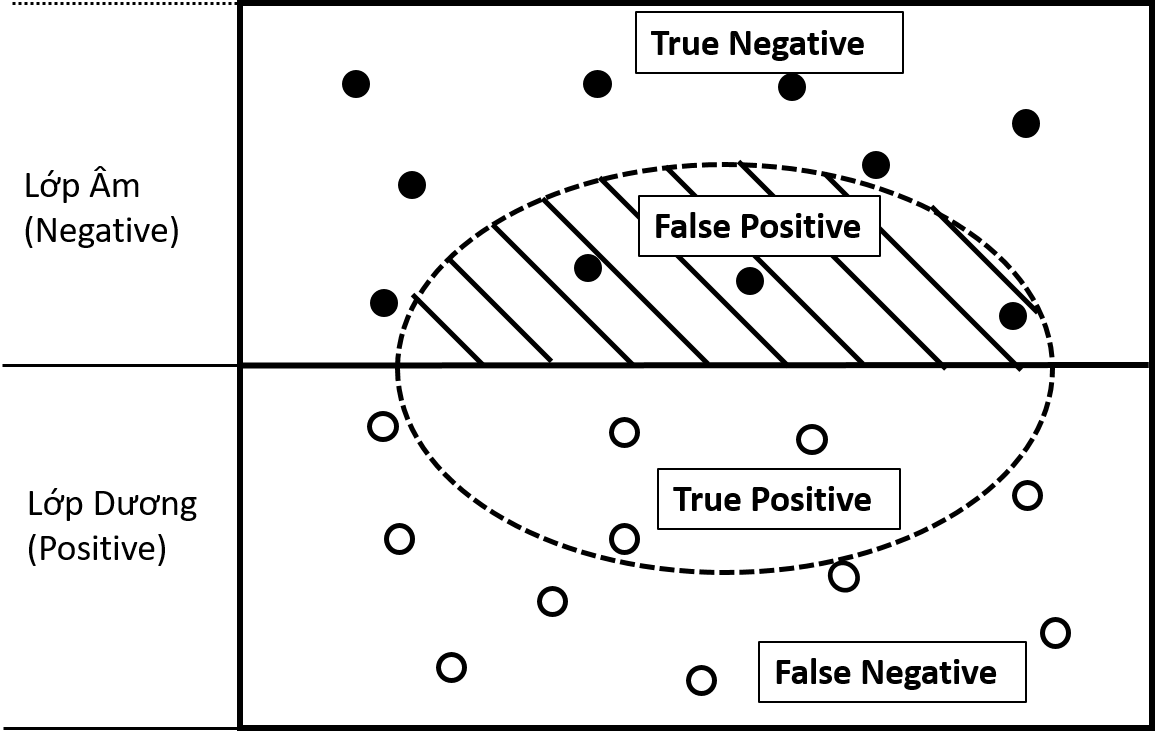
\includegraphics[scale=0.35]{../hinh/phepdo.png}
{\footnotesize \\
\begin{description}[noitemsep]
\item[Hình chữ nhật] Toàn bộ dữ liệu 
\item[Hình eclip] Phần dữ liệu hệ thống cho rằng thuộc lớp Positive
\item[True Negative] Phần dữ liệu thuộc lớp Negative, hệ thống cũng cho rằng thuộc lớp Negative
\item[False Negative] Phần dữ liệu thuộc lớp Positive, hệ thống cho rằng thuộc lớp Negative
\item[True Positive] Phần dữ liệu thuộc lớp Positive, hệ thống cũng cho rằng thuộc lớp Positive
\item[False Positive] Phần dữ liệu thuộc lớp Negative, hệ thống cho rằng thuộc lớp Positive
\end{description}
\par}
\end{minipage}
\caption{Các thành phần trong các phép đo Độ chính xác, Độ bao phủ và f1}
\label{fig:phepdo}
\end{figure}

Dựa trên câu trả lời là tập hợp các phần tử mà hệ thống cho rằng thuộc lớp dương, toàn bộ dữ liệu sẽ được chia thành 4 nhóm như Hình \ref{fig:phepdo}. Từ đó, định nghĩa các phép đo như sau:
\subsubsection*{Độ chính xác (Precision)}
Độ chính xác \(P\) là hệ số đánh giá mức độ chính xác của câu trả lời, mức độ chính xác càng cao thì giá trị \(P\) càng lớn. Công thức tính \(P\) như sau:
$$P=\frac{\text{Tổng số câu trả lời đúng hệ thống đưa ra}}{\text{Tổng số câu trả hệ thống đưa ra}} = \frac{\text{|True Positive|}}{\text{|True Positive| + |False Positive|}}$$
Trong trường hợp tất cả những câu trả lời hệ thống đưa ra đều đúng, thì giá trị $P=1$ là lớn nhất. Quy ước rằng nếu hệ thống không đưa ra câu trả lời nào, khi đó ngầm hiểu hệ thống không "sai", giá trị $P=1$.
\subsubsection*{Độ bao phủ (Recall)}
Độ bao phủ \(R\) là hệ số đánh giá mức độ bao phủ của các câu trả lời, độ bao phủ càng cao thì \(R\) càng lớn. Công thức tính \(R\) như sau:
$$R=\frac{\text{Tổng số câu trả lời đúng hệ thống đưa ra}}{\text{Tổng số câu trả lời đúng thực tế}} = \frac{\text{|True Positive|}}{\text{|True Positive| + |False Negative|}}$$
Trong trường hợp hệ thống đưa ra đủ tất cả các câu trả lời đúng thì giá trị $R=1$ là lớn nhất.
\subsubsection*{F-measure}
Trên thực tế, với lượng dữ liệu lớn và phức tạp, khả năng tất cả những câu trả lời hệ thống đưa ra đều đúng và hệ thống đưa ra đủ tất cả các câu trả lời đúng ($P=R=1$) là rất thấp. Hai hệ số này thường bù trừ lẫn nhau, tức là để đạt độ bao phủ \(R\) cao, hệ thống có xu hướng đưa ra nhiều câu trả lời hơn làm cho xác suất có câu trả lời sai tăng, độ chính xác \(P\)  giảm, và ngược lại. Một hệ thống nếu chỉ có \(P\) cao mà \(R\) thấp thì tuy hệ thống có câu trả lời thường đúng nhưng lại bỏ sót nhiều trường hợp đúng khác. Hệ thống chỉ có \(R\) cao mà \(P\) thấp thì hệ thống đó tuy bao quát đầy đủ tất cả các trường hợp đúng thực tế, nhưng tỉ lệ câu trả lời sai lại lớn. Một hệ thống tốt yêu cầu cả độ chính xác P và độ bao phủ đều cao R. Do đó vấn đề đặt ra là tìm một độ đo duy nhất mà đảm bảo cả \(P\) và \(R\) để thuận tiện cho việc tối ưu.\\

Để giải quyết vấn đề trên, ta sử dụng tiêu chí đánh giá \(F\) là trung bình điều hòa của \(P\) và \(R\), từ đó đảm bảo rằng chỉ khi cả \(P\) và \(R\) cao thì \(F\) mới đạt giá trị cao. Công thức tính \(F\) như sau:
$$F=2*\frac{P*R}{P + R} $$
\subsubsection*{Độ chính xác (P), độ bao phủ (R), F đối với bài toán phân loại đa lớp}
Để áp dụng 3 độ đo trên vào bài toán phân loại 3 lớp, chúng tôi xem như đang giải 3 bài toán con thuộc loại bài toán phân loại nhị phân. Khi đó, điểm số của bài toán lớn bằng trung bình có trọng số của điểm số từng bài toán con. Cụ thể:
Xét 3 bài toán con:
\begin{enumerate}
\item Phân loại một câu thuộc lớp \tichcuc hay không thuộc lớp \tichcuc. Lớp dương được chọn là lớp \tichcuc
\item Phân loại một câu thuộc lớp \tieucuc hay không thuộc lớp \tieucuc. Lớp dương được chọn là lớp \tieucuc
\item Phân loại một câu thuộc lớp \trungtinh hay không thuộc lớp \trungtinh. Lớp dương được chọn là lớp \trungtinh
\end{enumerate}
Khi đó:
$$P = \alpha_1*P_1 + \alpha_2*P_2 + \alpha_3*P_3$$
$$R = \alpha_1*R_1 + \alpha_2*R_2 + \alpha_3*R_3$$
$$F = \alpha_1*F_1 + \alpha_2*F_2 + \alpha_3*F_3$$
với $\alpha_1 + \alpha_2 + \alpha_3 = 1$ và $\alpha_1, \alpha_2, \alpha_3$ lần lược là tỉ lệ số lượng các câu thuộc lớp \tichcuc, \tieucuc, \trungtinh trong tập dữ liệu huấn luyện.
\subsubsection*{K-fold cross validation}
Sau khi đã có thước đo \(F\), chúng tôi đề xuất sử dụng phương pháp \textit{k-fold cross validation} để đánh giá hiệu quả của hệ thống. Phương pháp này nhằm tránh trường hợp tập kiểm tra, vì được chia ngẫu nhiên, có thể rơi vào trường hợp quá dễ hoặc quá khó đối với hệ thống. Tập dữ liệu được chia ngẫu nhiên thành \(k\) phần. Phần thứ \(i\) sẽ được chọn làm tập để đánh giá, \(k-1\) phần còn lại dùng cho việc học các tham số của mô hình. Tiến trình trên được thực hiện \(k\) lần với \(i\) chạy từ 1 đến \(k\), giá trị trung bình là kết quả cuối cùng dùng để đánh giá hệ thống.

\subsection{Thu thập và đánh giá dữ liệu} \label{sec:thu-thap-va-danh-gia-du-lieu}
\subsubsection*{Thu thập dữ liệu}
%Bảng dữ liệu mẫu gồm id và sen, mỗi sen có id duy nhất
Trong nghiên cứu này, chúng tôi thu thập dữ liệu từ \term{website} PubMed \footnote{https://www.ncbi.nlm.nih.gov/pubmed}. Trang web cung cấp miễn phí tóm tắt (\term{abstract}) của các bài báo khoa học trong lĩnh vực y khoa. Phần tóm tắt của các bài báo không có cấu trúc chung, chúng tôi chỉ thu thập những tóm tắt nào có chứa phần kết luận (\term{Conclusion}) như Hình \ref{fig:bai-bao-mau}. Dựa theo báo cáo \cite{sarker2011outcome} gợi ý rằng sử dụng những câu kết luận giúp tăng hiệu quả phân loại, chúng tôi chỉ giữ lại phần Kết luận, và sử dụng công cụ tìm kiếm cùng bộ lọc để tìm các bài có loại xuất bản (\term{publication type}) là ``clinical trial''.\\

Vì \term{website} PubMed không chính thức hỗ trợ cung cấp dữ liệu, chúng tôi tự hiện thực công cụ phục vụ nhu cầu này. TODO mô tả thêm\\

Sau khi chạy công cụ trên, kết quả thu được là những đoạn văn thuộc phần kết luận. Bản thân việc phân tách câu trong đoạn cũng là 1 bài toán, thường được gọi là Định hướng ranh giới câu (\term{Sentence boundary disambiguation}), không nằm trong phạm vi đề tài. Trong luận án này, chúng tôi sử dụng giải thuật phân tách câu Punkt sentence segmenter \cite{kiss2006unsupervised} được hiện thực trong thư viện NLTK. Dữ liệu chúng tôi thu thập được gồm 1182 câu được gán mã số (\term{Id}) tuần tự và lưu trữ như Bảng \ref{table:data}.
\begin{figure}[H]
\centering
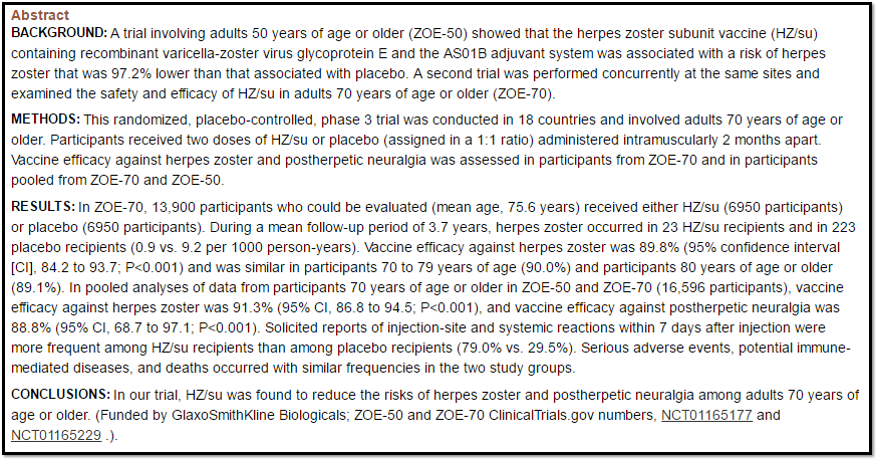
\includegraphics[scale=0.7]{../hinh/bai_bao_mau.png}
\caption{Tóm tắt của 1 bài báo} \label{fig:bai-bao-mau}
\end{figure}

\begin{table}[H]
\centering
\begin{minipage}{1.0\textwidth}
\caption{Một số mẫu từ tập dữ liệu sau khi thu thập} \label{table:data}
\begin{tabular}{|l| m{0.9\textwidth} | } 
\hline
\textbf{Id} & \textbf{Sentence} \\ \hline
10 & This study was a negative study, though there was a suggestion of benefit of methylprednisolone acetate in a population of young adults with acute radicular low back pain. \\ \hline
17 & Data extraction and analyses and quality assessment were conducted according to the Cochrane standards. \\ \hline
36 & Patients subjectively reported significantly greater relief from symptoms with Debacterol than with Kenalog-in-Orabase or no treatment. \\ \hline
\end{tabular}
\end{minipage}
\end{table}

\subsubsection*{Đánh nhãn dữ liệu}
Giải thuật học máy chúng tôi sử dụng là có giám sát nên dữ liệu đầu vào cần được đánh nhãn phân loại tính phân cực cảm xúc (\tichcuc, \tieucuc, \trungtinh) trước khi đưa vào học và kiểm tra. Vì vậy, chúng tôi đã hiện thực một trang web phục vụ cho việc đánh nhãn dữ liệu.\\

\begin{figure}[h]
\centering
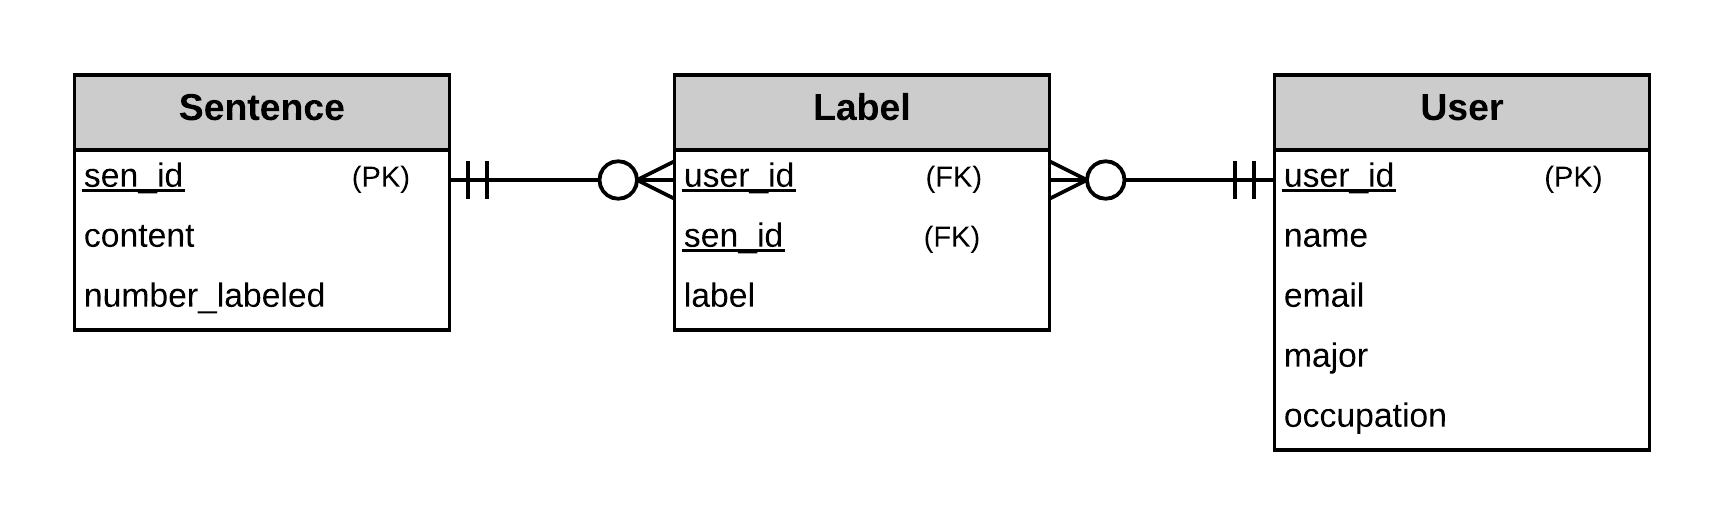
\includegraphics[scale=0.25]{../hinh/EERD.png}
\caption{Mô hình thực thể liên kết tăng cường của cơ sở dữ liệu}
\label{fig:SQL}
\end{figure}

Đầu tiên, chúng tôi sử dụng MySQL Workbench 6.3 \footnote{http://www.mysql.com/products/workbench/} để tạo cơ sở dữ liệu lưu trữ theo lược đồ ở Hình \ref{fig:SQL}:
\begin{itemize}
\item Bảng \myquote{Sentence} chứa dữ liệu các câu gồm mã số câu (\myquote{sen\_id}), nội dung câu (\myquote{content}) và số lần câu được đánh nhãn (\myquote{number\_labeled}). Tập dữ liệu sau khi thu thập sẽ được thêm vào bảng này với giá trị số lần câu được đánh nhãn ở mỗi câu ban đầu mặc định bằng 0.
\item Bảng \myquote{Submission} chứa nhật ký đánh nhãn gồm mã số nhãn (\myquote{id}) tăng tuần tự theo mỗi nhãn được đánh cho một câu bất kỳ, mã số câu (\myquote{sentence\_id}) tương ứng với mã số câu ở Bảng \myquote{Sentence}, loại nhãn (\myquote{label}) với quy ước giá trị 0, 1, 2 lần lượt tương ứng cho các nhãn \tieucuc, \trungtinh, \tichcuc.
\end{itemize}

\begin{figure}[H]
\centering
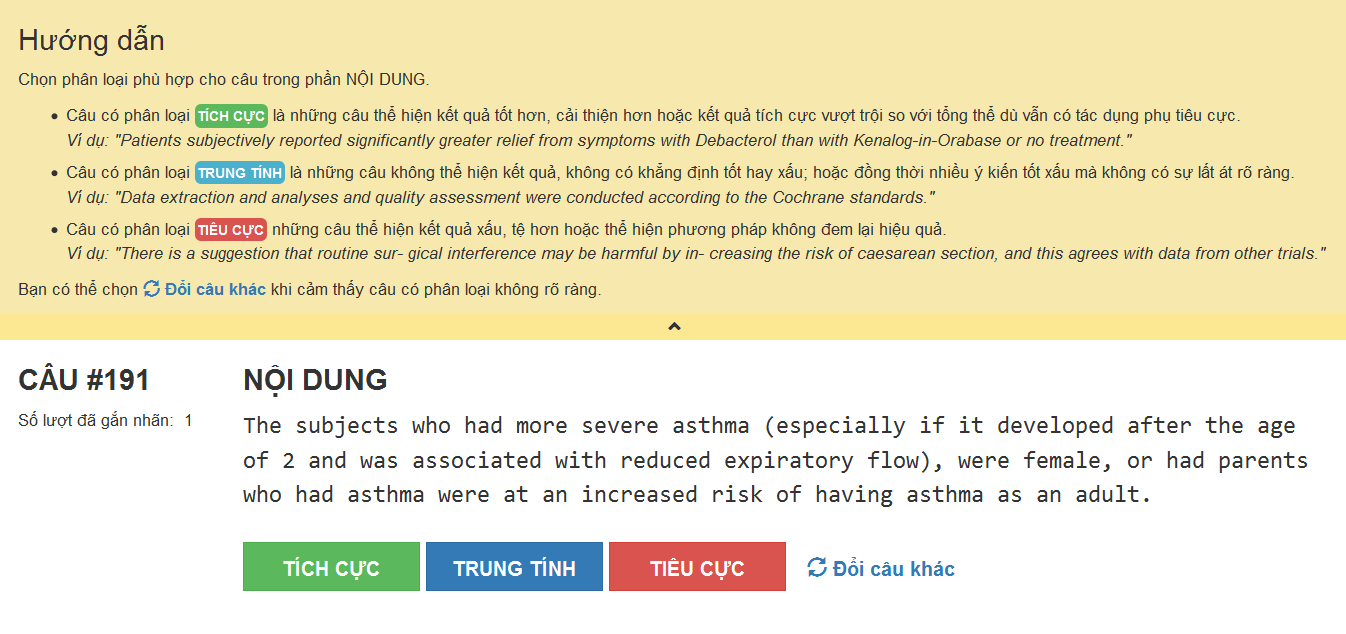
\includegraphics[scale=0.45]{../hinh/Webpage.png}
\caption{Giao diện trang đánh nhãn dữ liệu}
\label{fig:web}
\end{figure}

Tiếp theo, chúng tôi xây dựng một trang web hỗ trợ người dùng đánh nhãn dữ liệu\footnote{http://anotation.mybluemix.net/}. Giao diện web đơn giản, trực quan (Hình \ref{fig:web}), gồm hai phần chính:
\begin{itemize}
\item Phần hướng dẫn: mô tả cách sử dụng trang web để đánh nhãn dữ liệu, trong đó đặc tả chi tiết thế nào là phân loại \tichcuc, \tieucuc hay \trungtinh, lấy ví dụ cụ thể để người đọc dễ hình dung và hiểu rõ ràng về các loại nhãn phân loại.
\item Phần đánh nhãn: hiển thị thông tin một câu ngẫu nhiên thuộc bảng \myquote{Sentence} trong cơ sở dữ liệu và các lựa chọn để người dùng đánh nhãn phân loại. 
\end{itemize}

\begin{figure}[h]
\centering
\fbox{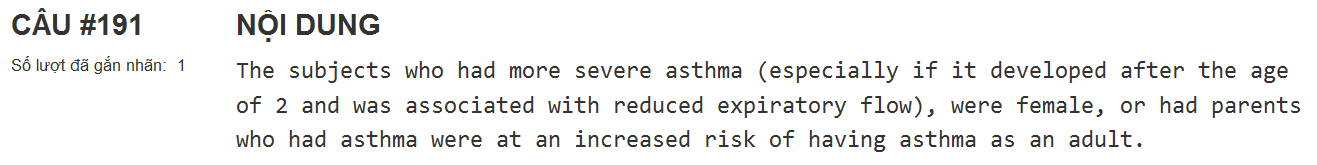
\includegraphics[scale=0.45]{../hinh/WebSenId.png}}
\caption{Thông tin một bản ghi thuộc bảng \myquote{Sentence}}
\label{fig:websen}
\end{figure}

Thông tin chi tiết một câu được hiển thị như Hình \ref{fig:websen} bao gồm giá trị các trường thuộc bảng \myquote{Sentence} (mã số câu, nội dung câu, số lần câu được đánh nhãn). Để gắn nhãn phân loại cho câu, người dùng sử dụng nhóm nút chức năng (Hình \ref{fig:webbtn}) gồm nút \textsc{tích cực} (gắn nhãn \tichcuc), nút \textsc{trung tính} (gắn nhãn \trungtinh), nút \textsc{tiêu cực} (gắn nhãn \tieucuc) hoặc lựa chọn ``Đổi câu khác'' nếu người dùng cảm thấy câu có phân loại không rõ ràng.

\begin{figure}[h]
\centering
\fbox{
\includegraphics[scale=0.45]{../hinh/WebLabel.png}}
\caption{Nhóm nút chức năng hỗ trợ người dùng lựa chọn phân loại}
\label{fig:webbtn}
\end{figure}

Quy trình gắn nhãn dữ liệu của trang web được mô hình hóa như Hình \ref{fig:updatedb}. Mỗi lần người dùng mới truy cập hoặc tải lại trang web, hệ thống lựa chọn ngẫu nhiên một câu trong dữ liệu để hiển thị. Khi người dùng đánh nhãn \tichcuc, \tieucuc hoặc \trungtinh cho câu, cơ sở dữ liệu sẽ cập nhật dữ liệu trong bảng \myquote{Sentence}: tăng thêm 1 cho số lần câu được đánh nhãn với mã số câu tương ứng, đồng thời thêm một bản ghi vào bảng \myquote{Submission} với mã số câu tương ứng kèm lựa chọn phân loại của người dùng (chỉ lưu các giá trị 0, 1, 2). Nếu người dùng chọn ``Đổi câu khác'' hệ thống không cập nhật mà chỉ hiển thị ngẫu nhiên một câu khác trong tập dữ liệu để người dùng tiến hành gán nhãn.

Sau khi hoàn thành trang web đánh nhãn dữ liệu, chúng tôi đã tiến hành gắn nhãn cho tập dữ liệu. Kết quả tập dữ liệu sau khi gắn nhãn được lưu lại như Bảng \ref{table:labeleddata}.

%Sau khi hoàn thành trang web đánh nhãn dữ liệu, chúng tôi đã nhờ 14 bạn hiện đang học tập và nghiên cứu tại trường Đại học Y Dược thành phố Hồ Chí Minh hỗ trợ gắn nhãn cho tập dữ liệu. Bước tiếp theo, chúng tôi tiến hành lọc kết quả đã gắn nhãn như sau:

%\begin{itemize}
%\item Với những câu chỉ có 1 loại nhãn được gắn: lưu kết quả xem như là nhãn phân loại cuối cùng của câu.
%\item Với những câu có 2 loại nhãn được gắn: tự chỉnh sửa, lấy kết quả đúng lưu như nhãn phân loại cuối cùng của câu.
%\item Với những câu có 3 loại nhãn được gắn: bỏ những câu này ra khỏi tập dữ liệu vì nghi ngờ độ nhập nhằng về ý nghĩa phân cực của câu.
%\end{itemize}

%Kết quả sau khi lọc được lưu lại như Bảng \ref{table:labeleddata}.

\begin{table}[H]
\centering
\begin{minipage}{1.0\textwidth}
\caption{Một số mẫu từ tập dữ liệu sau khi đánh nhãn} \label{table:labeleddata}
\label{table:labeleddata}
\begin{tabular}{ |c|p{0.83\textwidth}|l| } 
 \hline
 \textbf{Id} & \textbf{Sentence} & \textbf{Label} \\ 
 \hline
 10 & This study was a negative study, though there was a suggestion of benefit of methylprednisolone acetate in a population of young adults with acute radicular low back pain. & 0\\ \hline
 17 & Data extraction and analyses and quality assessment were conducted according to the Cochrane standards. & 1\\ \hline
 36 & Patients subjectively reported significantly greater relief from symptoms with Debacterol than with Kenalog-in-Orabase or no treatment. & 2\\ 
 \hline
\end{tabular}
\end{minipage}
\end{table}

\begin{figure}[H]
\centering
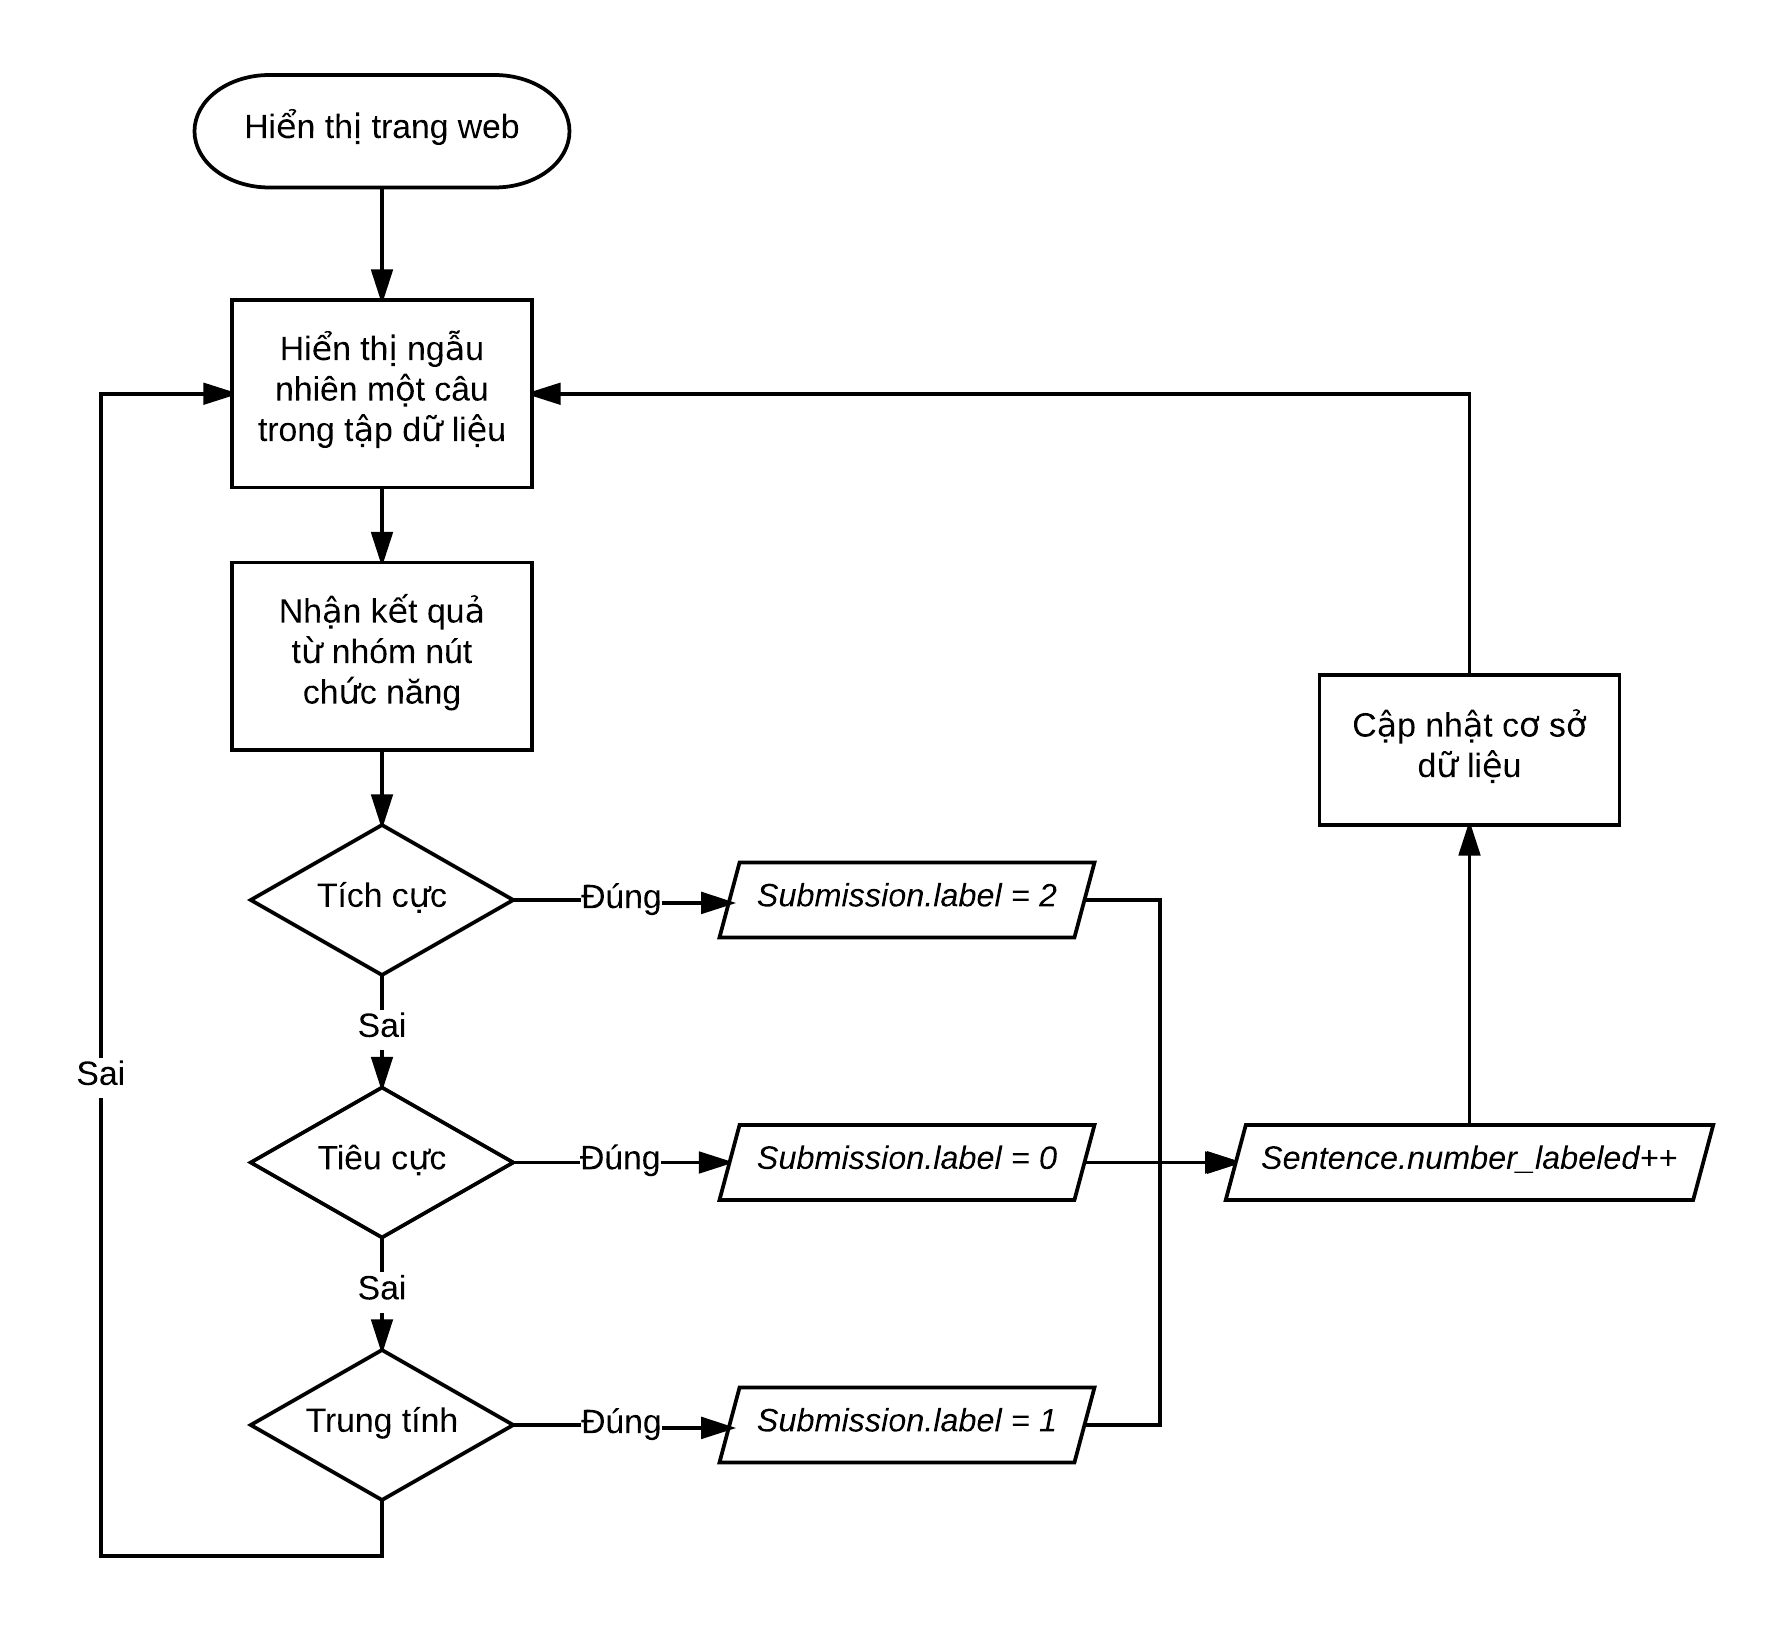
\includegraphics[scale=0.27]{../hinh/UpdateDatabase.png}
\caption{Quy trình xử lý gắn nhãn dữ liệu của trang web}
\label{fig:updatedb}
\end{figure}

\subsubsection*{Đánh giá dữ liệu}
TODO nhờ bao nhiêu người...
Sau khi xây dựng trang web hỗ trợ đánh nhãn, chúng tôi đã thu thập được 161 câu được đánh nhãn. Chúng tôi sử dụng phương pháp đánh giá độ đồng nhất Flessi Kappa với các tham số: $m=2, n=46, k=3$, kết quả $\kappa = 36.91\% $. Điểm số này thể hiện độ đồng nhất thuộc mức vừa (\term{fair argreement}). Kết quả này còn thấp so với nghiên cứu \cite{sarker2011outcome} (70.6\%). Điều này xảy ra vì sự nhập nhằng về ý nghĩa của 1 số câu và sự hiểu không đồng nhất trong quy ước về tính \tichcuc, \tieucuc, \trungtinh giữa các bạn đánh nhãn. Để giải quyết, 2 thành viên trong nhóm chúng tôi tự đánh nhãn các câu còn lại.  Kết quả $\kappa=72.54\%$ được tính trên 100 câu được 2 người đánh nhãn. Kết quả trên được xem khá tốt (\term{substantial agreement})

\subsection{Kết quả thí nghiệm} \label{subsec:ket-qua-thi-nghiem}
Với mỗi lần chạy, chúng tôi sử dụng k-fold với $k=5$. Tuy nhiên, do tập dữ liệu không đủ lớn, kết quả các lần chạy có sự dao động, vì vậy, với mỗi lần thử nghiệm, chúng tôi lặp lại việc chạy k-fold 30 lần, sau đó lấy điểm số trung bình xem như kết quả cuối cùng. Đối với giải thuật học máy SVM, có 2 tham số cần được tùy chỉnh thích hợp. Để xác định tham số c, hệ thống chạy nhiều lần với c thuộc 1 khoảng cho trước (trong nghiên cứu này, c chạy từ 20 đến 30), từ đó chọn ra giá trị c tương ứng với độ đo f lớn nhất. Như vậy, với mỗi thử nghiệm, giá trị độ do f luôn là giá trị cao nhất được chọn từ những lần chạy với giá trị c thay đổi từ 20 đến 30. \\

Trong mục này chúng tôi trình bày 4 nhóm thử nghiệm: Thử nghiệm với đặc trưng n-gram, thử nghiệm với đặc trưng phủ định, thử nghiệm kết hợp các đặc trưng cơ bản và thử nghiệm kết hợp các đặc trưng cơ bản với đặc trưng mở rộng SO-CAL
\subsubsection*{Thử nghiệm với đặc trưng n-gram}
Chúng tôi tiến hành thử nghiệm với đặc trưng n-gram trước tiên vì như đã phân tích ở mục \ref{sec:ngram}, n-gram được xem như đặc trưng nền tảng (baseline). Kết quả thử nghiệm thể hiện ở Bảng \ref{table:ngram}
\begin{table}[H]
\centering
\begin{minipage}{1.0\textwidth}
\caption{Các thử nghiệm nhằm tối ưu hóa đặc trưng n-gram} \label{table:ngram}
\begin{tabular}{|l| m{0.5\textwidth} | >{\centering\arraybackslash} m{0.1\textwidth} | >{\centering\arraybackslash}m{0.1\textwidth} | >{\centering\arraybackslash}m{0.1\textwidth} | } 

\hline
\textbf{STT} & \textbf{Đặc trưng} & \textbf{P (\%)} & \textbf{R (\%)} & \textbf{F (\%)} \\ \hline
1 & Unigram (F, min\_df = 1) & 66.21 & 65.46 & 65.06 \\ %\hline
2 & Unigram (P, min\_df = 1) & 66.56 & 65.62 & 65.23 \\ %\hline
3 & Unigram (F, min\_df = 2) & 66.50 & 65.55 & 65.59 \\ %\hline
4 & Unigram (P, min\_df = 2) & 68.26 & 67.38 & 67.31 \\ %\hline
5 & Unigram (F, min\_df = 3) & 66.98 & 65.48 & 65.80 \\ %\hline
6 & Unigram (P, min\_df = 3) & 68.12 & 67.23 & 67.32 \\ 
7 & Unigram (F, min\_df = 4) & 67.02	& 65.13 & 65.62 \\ 
8 & Unigram (P, min\_df = 4) & 67.83 & 66.34 & 66.71 \\% \hline
9 & Unigram (F, min\_df = 5) & 66.75 & 64.21 & 64.92 \\ 
10 & Unigram (P, min\_df = 5) & 67.18 & 65.27 & 65.79 \\ \hline
11 & Unigram + Bigram (P, min\_df  = 3) & 68.72 & 67.83 & 67.77 \\% \hline
12 & Unigram  + Bigram + Trigram \newline (P, min\_df = 3) & 68.68 & 68.00 & 67.87 \\ 
13 &  \textbf{Unigram  + Bigram + Trigram + 4-gram}\textbf{(P, min\_df = 3)} & \textbf{68.76} & \textbf{68.09} & \textbf{67.96}\\ 
14  &  Unigram  + Bigram + Trigram + 4-gram + 5-gram (P, min\_df = 3) & 68.81 & 67.98 & 67.86 \\ \hline
\end{tabular}
{\footnotesize \\
\begin{description}[noitemsep]
\item[P] Chỉ quan tâm đến việc có xuất hiện hay không n-gram trong câu, nhận 2 giá trị: 1 hoặc 0
\item[F] Quan tâm đến số lần xuất hiện n-gram trong câu
\item[min\_df] Số câu có n-gram đó để n-gram đó được thêm vào bộ từ vừng
\end{description}
\par}
\end{minipage}
\end{table}

Các thử nghiệm từ 1-10 cho thấy 2 xu hướng. Hình \ref{fig:mindf-p-f} thể hiện sự phụ thuộc của độ đo F vào tham số $min\_df$ và cách vector hóa đặc trưng n-gram. $min\_df$ là tham số ngưỡng, chỉ những n-gram nào có số lần xuất hiện từ $min\_df$ trở lên mới được thêm vào tập từ vựng S. Qua biểu đồ có thể thấy, với $min\_df$ quá nhỏ hoặc quá lớn đều làm giảm giá trị độ đo F. Khi $min\_df$ quá nhỏ, số lượng từ vựng quá lớn dẫn tới số lượng ngram gây nhiễu nhiều. Ngược lại khi $min\_df$ quá lớn, tập từ vựng quá nhỏ dẫn tới có quá ít thông tin trong câu được giữ lại, không đủ thông tin để phân loại. Từ biểu đồ, $min\_df=2$ hay $min\_df=3$ không có sự khác biệt rõ rệt giá trị độ đo F. Trong nghiên cứu này, chúng tôi chọn tham số $min\_df=3$ cho các thử nghiệm còn lại.\\

Hình \ref{fig:mindf-p-f} còn thể hiện một xu hướng khác. Kết quả của n-gram tốt hơn hẳn khi sử dụng phương pháp vector hóa nhị phân. Kết quả này phù hợp với báo cáo của \cite{pang2002thumbs}. Ngược lại, nghiên cứu \cite{sarker2011outcome} thực hiện phân tích cảm xúc trên đoạn văn bản, khẳng định không có sự khác biệt đáng kể giữa 2 cách vector hóa. Điều này có thể do việc lặp từ trên câu có ý nghĩa khác với lặp từ trên đoạn.\\

\begin{figure}[H]
\centering
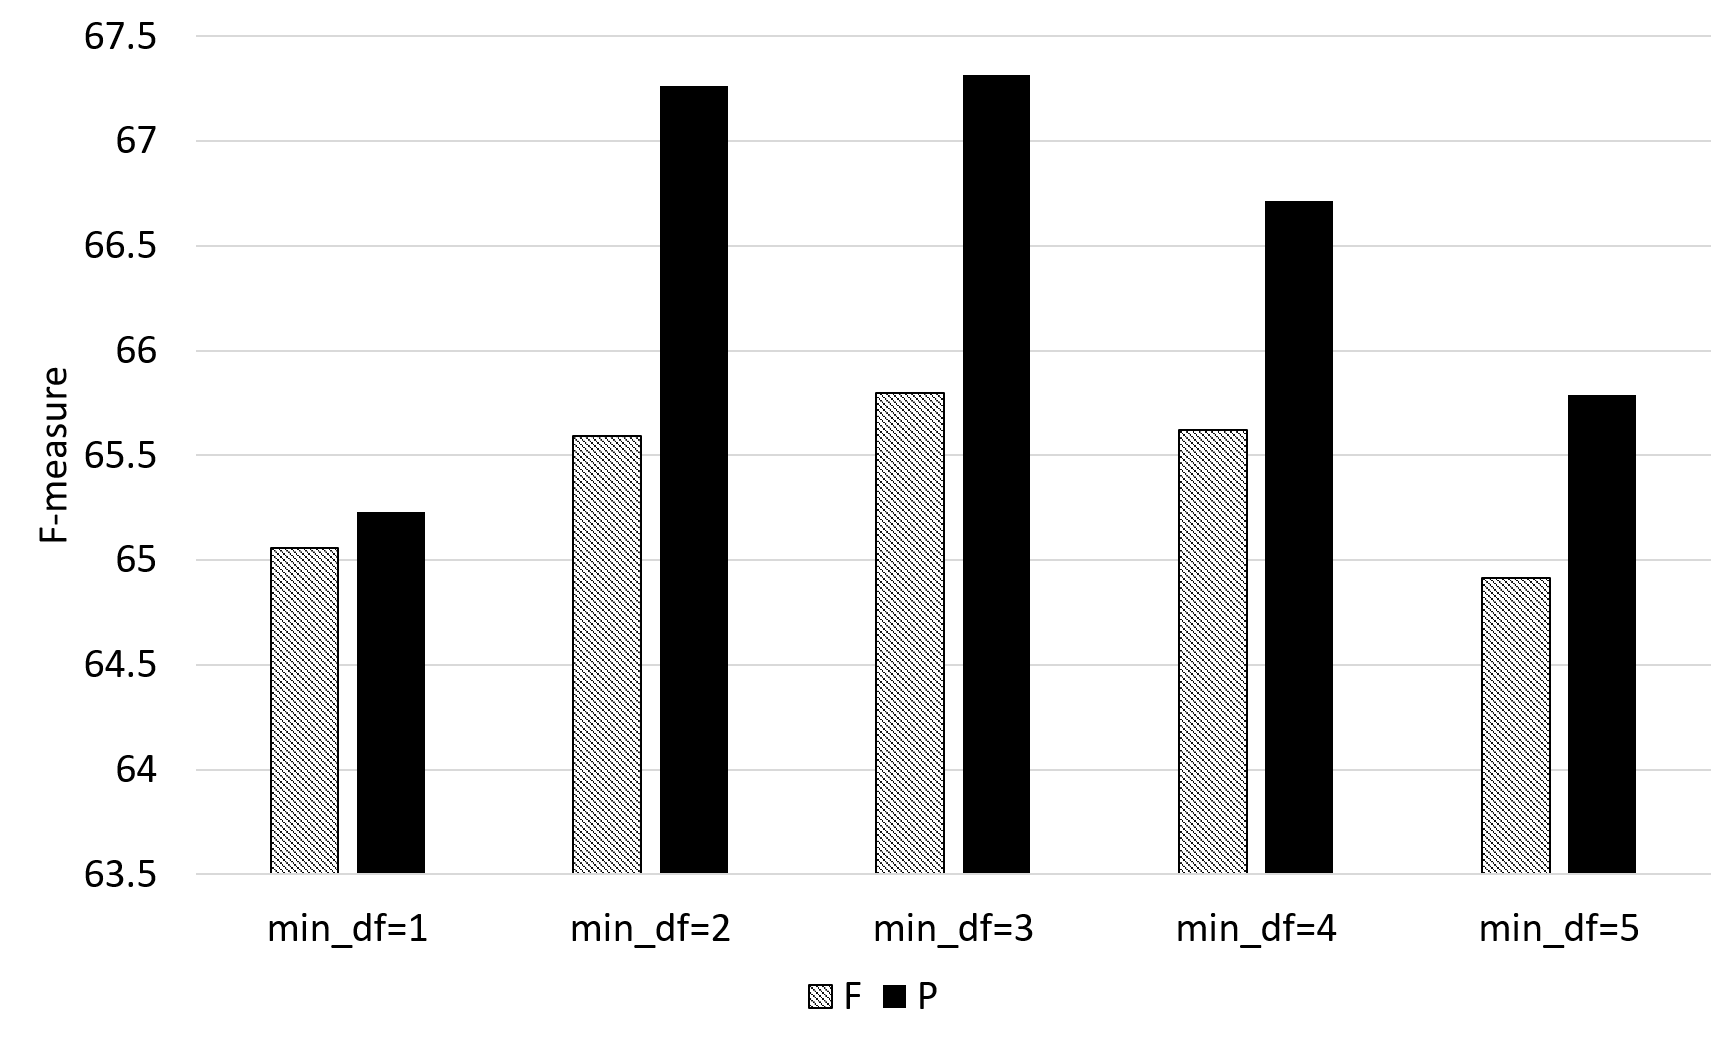
\includegraphics[scale=0.25]{../hinh/mindf_p_f.png}
\caption{Mối quan hệ giữa tham số min\_df, cách vector hóa và độ đo F} \label{fig:mindf-p-f}
\end{figure}

Hình \ref{fig:ket-hop-ngram} thể hiện ảnh hưởng của cách kết hợp các n-gram. Theo đó, có sự cải thiện khi chuyển từ việc chỉ dùng Unigram sang dùng kết hợp Unigram và Bigram. Khi mở rộng việc kết hợp đến $n=3$ và $n=4$, mặc dù chỉ số F có tăng không thực sự đáng kể. Khi kết hợp đến $n=5$, chỉ số F bắt đầu giảm. Với n càng lớn, mặc dù số lượng ngram không khác nhau nhiều (giả sử 1 câu có 20 từ, với $n=1$ tạo ra 20 ngram, $n=3$ tạo ra 18 ngram) nhưng các n-gram có tần suất xuất hiện càng thấp. Trong khi đó, hệ thống chỉ thêm ngram vào tập từ vựng S chỉ khi từ đó xuất hiện từ 3 lần trở lên. Vì vậy, việc kết hợp với các ngram (n lớn, $n=5$ chẳng hạn) không giúp bổ sung thêm vào tập từ vựng S. Ngược lại, với $n=2, 3, 4$ giúp hệ thống nhận thêm các cụm từ như: no evidence, improve quality life, reduce risk,... Trong các thử nghiệm tiếp theo, chúng tôi dùng đặc trưng n-gram là sự kết hợp của Unigram, Bigram, Trigram và 4-gram (ngram với $n=4$).
\begin{figure}[H]
\centering
\begin{minipage}{0.7\textwidth}
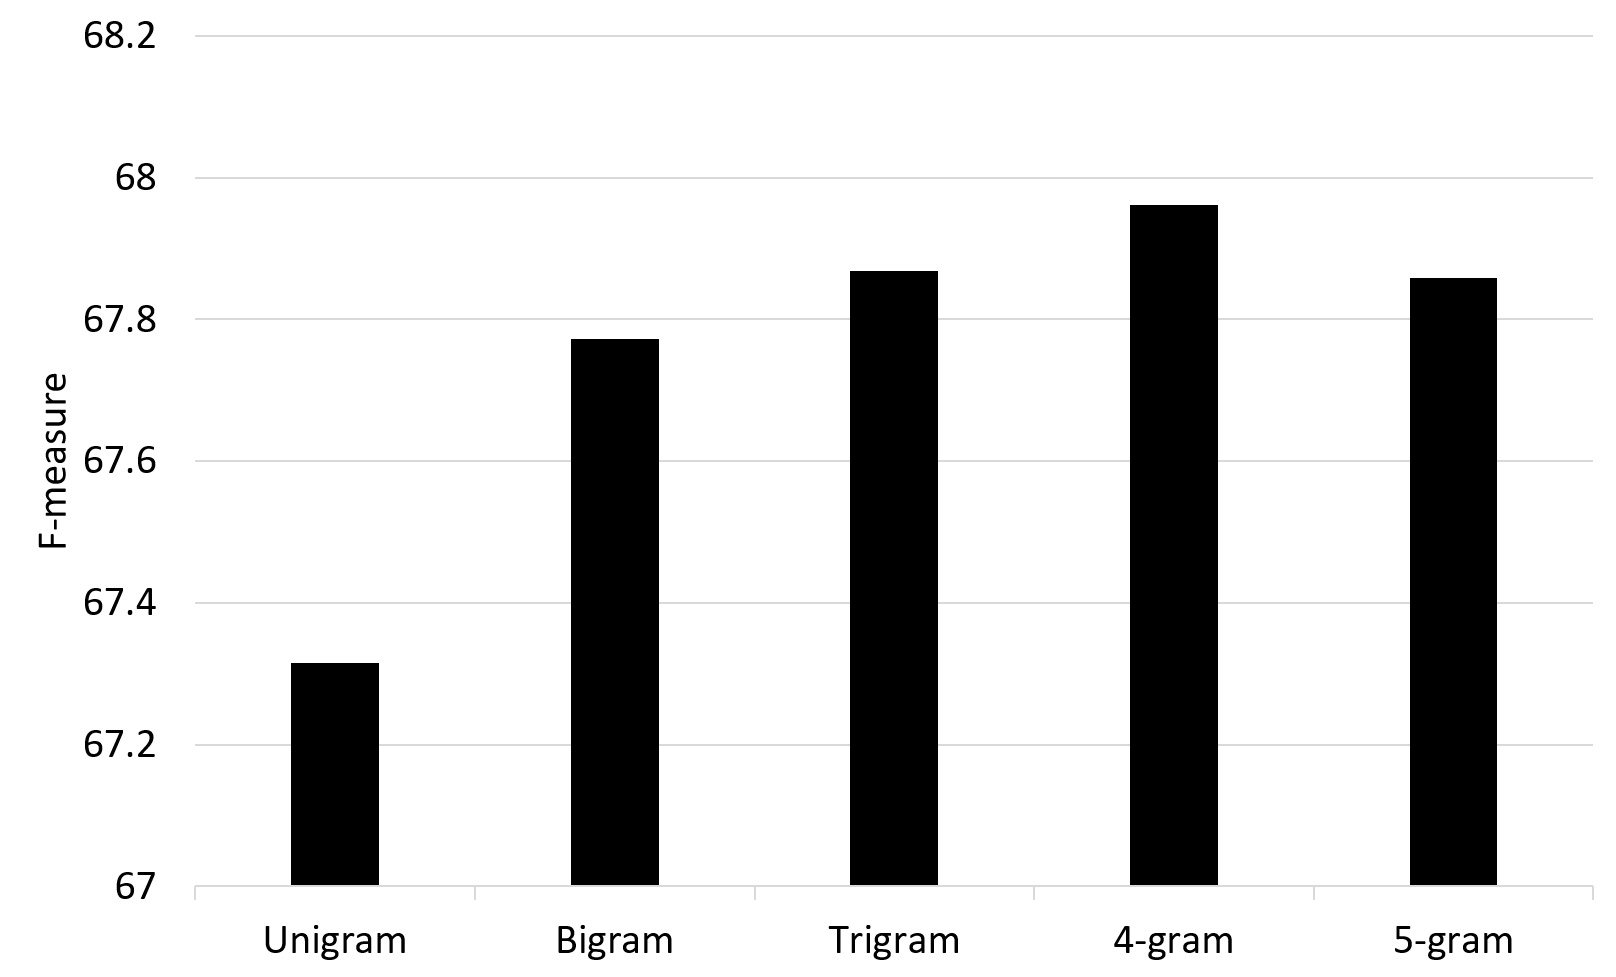
\includegraphics[scale=0.25]{../hinh/ket_hop_ngram.png}
{\footnotesize \\
Tên mỗi cột chỉ là đặc trưng ngram đại diện. Ví dụ: Trigram đại diện cho thử nghiệm thứ 12, là kết hợp cả Unigram, Bigram và Trigram \par}
\caption{Kết hợp các n-gram} \label{fig:ket-hop-ngram}
\end{minipage}
\end{figure}

\subsubsection*{Thử nghiệm với đặc trưng Phủ định}
Các thử nghiệm trong phần này đều dùng kết hợp với đặc trưng n-gram. Bảng \ref{table:negation} thể hiện hiệu quả của việc rút trích yếu tố phủ định qua 7 cách khác nhau, so sánh giữa 2 công cụ: Metamap sử dụng giải thuật NegEx và bản gốc NegEx. Trong 7 cách tích hợp yếu tố phủ định vào hệ thống, cách dùng của thí nghiệm 2 cho kết quả tốt nhất, xét cho cả 2 công cụ. Trong đó, NegEx bản gốc cho kết quả cao hơn. Chúng tôi sử dụng cách dùng như thí nghiệm 2 và công cụ NegEx bản gốc cho thí nghiệm ở phần sau.
\begin{table}[H]
\centering
\begin{minipage}{1\textwidth}
\caption{Các thử nghiệm nhằm tối ưu đặc trưng Phủ định} \label{table:negation}
\begin{tabular}{|l|m{0.3\textwidth}|ccc|ccc|}
\hline
\multirow{2}{*}{\textbf{STT}} & \multirow{2}{*}{\textbf{Đặc trưng}} & \multicolumn{3}{c|}{\textbf{Negation tu metamap}} & \multicolumn{3}{c|}{\textbf{Negation 2}}  \\ \cline{3-8}
                     &                            & \textbf{P}           & \textbf{R}           & \textbf{F}           & \textbf{P}        & \textbf{R}        & \textbf{F}        \\
\hline
1 & Kiểm tra trong câu có yếu tố phủ định hay không& 69.36 & 68.53 & 68.45 &
69.59 & 68.32 & 68.50 \\ \hline

\textbf{2} & \textbf{Thay các từ phủ định trong câu bằng nhãn NEGATION} & \textbf{69.57} & \textbf{68.67} & \textbf{68.60} & 
\textbf{70.07} & \textbf{68.98} & \textbf{69.09} \\ \hline

3 & Thêm nhãn ``\_NEG'' ngay sau các từ chịu ảnh hưởng phủ định & 68.93 & 67.91 & 67.88 &
69.11 & 68.12 & 68.03 \\ \hline

4 & Kết hợp 1 và 2 & 68.88 & 68.10 & 68.09 &
69.95 & 68.64 & 68.82 \\ \hline

5 & Kết hợp 1 và 3 & 69.41 & 68.55  & 68.56 &
69.47 & 67.85 & 68.16 \\ \hline

6 & Kết hợp 2 và 3 & 68.84 & 68.02 & 67.93 &
69.00 & 68.00 & 67.83 \\ \hline

7 & Kết hợp 1 và 2 và 3 & 69.35 & 68.40 & 68.44 &
69.62 & 67.96 & 68.22 \\ \hline
\end{tabular}
%{\footnotesize \\
%\begin{description}[noitemsep]
%\item[P] Chỉ quan tâm đến việc có xuất hiện hay không n-gram trong câu, nhận 2 giá trị: 1 hoặc 0
%\item[F] Quan tâm đến số lần xuất hiện n-gram trong câu
%\item[min\_df] Số câu có n-gram đó để n-gram đó được thêm vào bộ từ vừng
%\end{description}
%\par}
\end{minipage}
\end{table}

\subsubsection*{Thử nghiệm kết hợp các đặc trưng cơ bản}
\begin{table}[H]
\centering
\begin{minipage}{1.0\textwidth}
\caption{Các thử nghiệm kết hợp các đặc trưng cơ bản} \label{table:ket-hop-dac-trung}
\begin{tabular}{|l| m{0.5\textwidth} | >{\centering\arraybackslash} m{0.1\textwidth} | >{\centering\arraybackslash}m{0.1\textwidth} | >{\centering\arraybackslash}m{0.1\textwidth} | } 
\hline
\textbf{STT} & \textbf{Đặc trưng} & \textbf{P} & \textbf{R} & \textbf{F} \\ \hline
1 & N-gram & 68.76 & 68.09 & 67.96  \\ \hline
2 & N-gram + \term{Change phrase} & 69.97 & 69.29 & 69.17\\ \hline
\textbf{3} & \textbf{N-gram + \term{Change phrase} + Phủ định} & \textbf{71.01} & \textbf{70.00} & \textbf{70.05}\\ \hline
4 & N-gram + \term{Change phrase} + Phủ định + Metamap & 70.88 & 70.00  & 69.99 \\ \hline
\end{tabular}
\end{minipage}
\end{table}
Bảng \ref{table:ket-hop-dac-trung} thể hiện kết quả khi kết hợp các đặc trưng cơ bản với nhau. \term{Change phrase} có hiệu quả rõ rệt khi giúp tăng 1.39\% so với \term{baseline} n-gram. Có thêm đặc trưng Phủ định góp phần cải thiện kết quả 2.15\%. Kết quả khi sử dụng n-gram với Metamap lại không cho kết quả tốt.
\subsubsection*{Thử nghiệm kết hợp các đặc trưng cơ bản với đặc trưng mở rộng SO-CAL}
\begin{table}[H]
\centering
\begin{minipage}{1\textwidth}
\caption{Các thử nghiệm kết hợp các đặc trưng cơ bản với đặc trưng mở rộng SO-CAL} \label{table:socal-ket-hop-dac-trung-khac}
\begin{tabular}{|l| m{0.5\textwidth} | >{\centering\arraybackslash} m{0.1\textwidth} | >{\centering\arraybackslash}m{0.1\textwidth} | >{\centering\arraybackslash}m{0.1\textwidth} | } 
\hline
\textbf{STT} & \textbf{Đặc trưng} & \textbf{P} & \textbf{R} & \textbf{F} \\ \hline
1 & N-gram + SO-CAL& 69.13 & 68.22 & 68.27 \\ \hline
2 & N-gram + Change\_Phrase + SO-CAL& 70.84 & 70.05 & 70.03 \\ \hline
\textbf{3} & \textbf{N-gram + Change\_Phrase + Negation + SO-CAL}& \textbf{71.64} & \textbf{70.70} & \textbf{70.74} \\ \hline
4 & N-gram + Change\_Phrase + Negation + UMLS + SO-CAL& 71.49 & 70.54 & 70.60 \\ \hline
\end{tabular}
\end{minipage}
\end{table}
Chúng tôi tiến hành thử nghiệm kết hợp đặc trưng mở rộng SO-CAL với các đặc trưng cơ bản, kết quả thể hiện ở Bảng \ref{table:socal-ket-hop-dac-trung-khac}. Xu hướng vẫn giống kết quả của Bảng \ref{table:ket-hop-dac-trung}: 2 đặc trưng Change\_Phrase và Negation khi kết hợp cùng SO-CAL đều giúp cải thiện kết quả (lần lượt là 1.76\% và 2.47\% so với n-gram kết hợp SO-CAL), tuy nhiên khi sử dụng n-gram kết hợp Metamap kết quả không có sự khác biệt.\\

Điểm khác biệt so với Bảng \ref{table:ket-hop-dac-trung} là có sự cải thiện trong từng lần thử nghiệm giữa tập các đặc trưng có SO-CAL và không có SO-CAL (Hình \ref{fig:socal-vs-co-ban}). Kết quả tốt nhất trong các thử nghiệm này, cũng là kết quả tốt nhất mà hệ thống chúng tôi đạt được là \textbf{70.74\%}.
\begin{figure}[H]
\centering
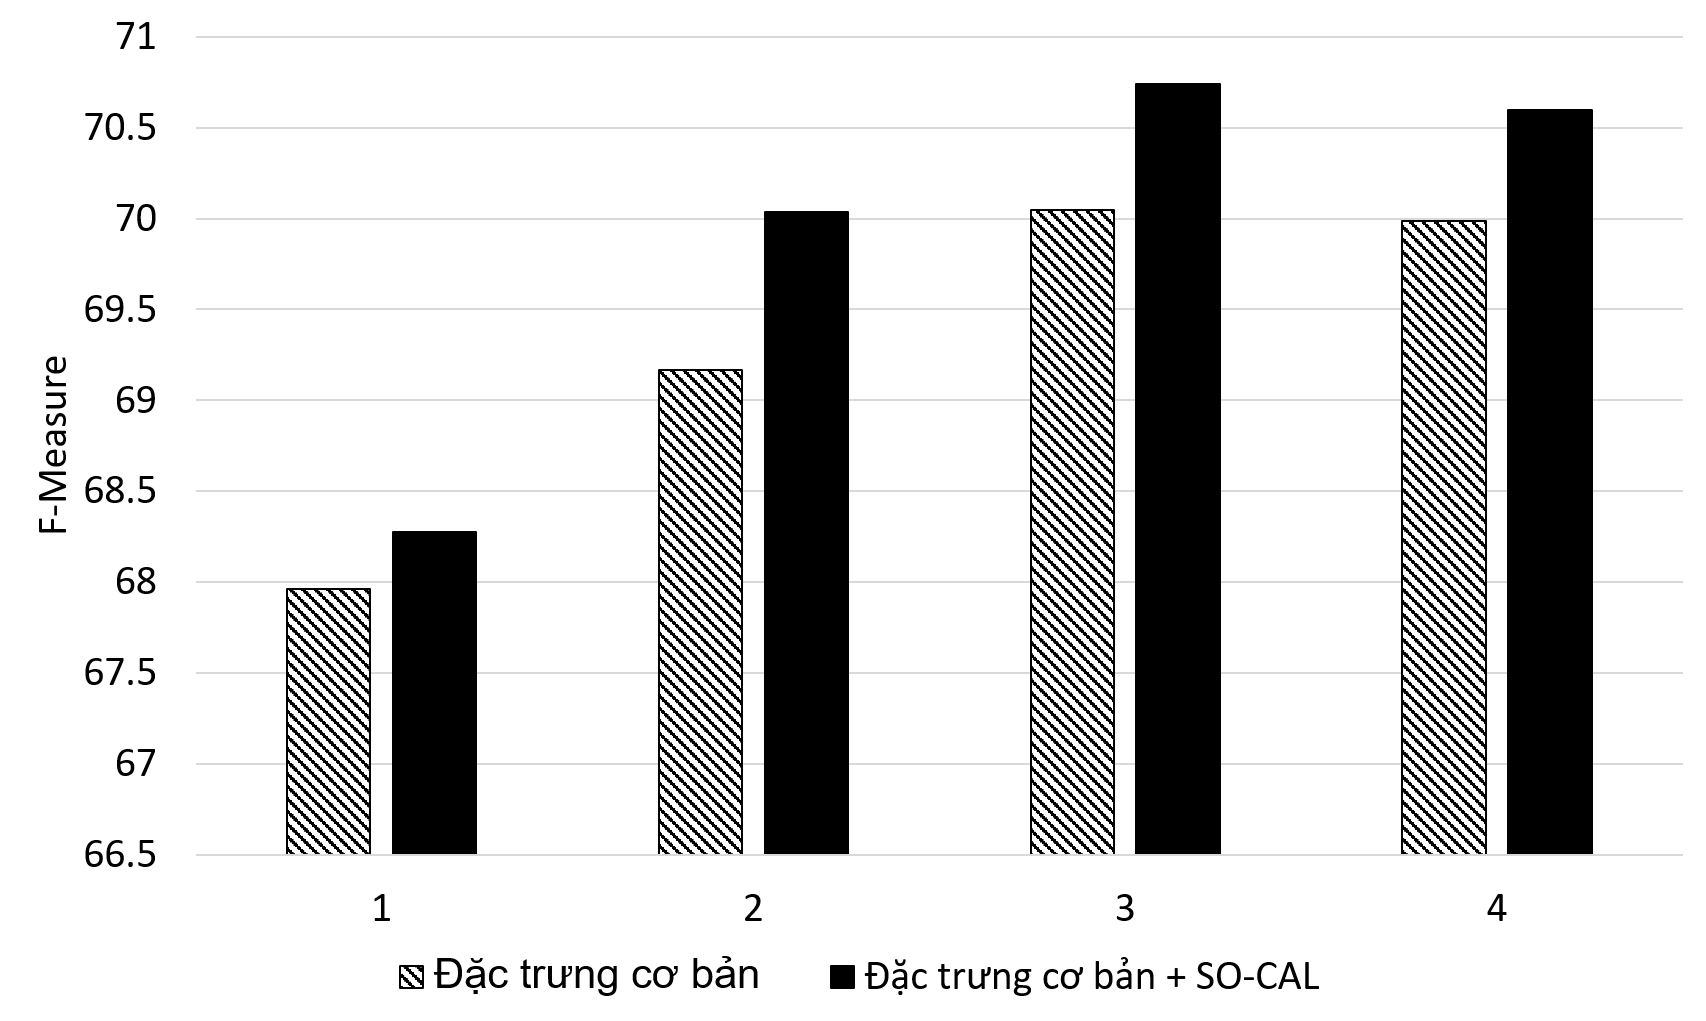
\includegraphics[scale=0.35]{../hinh/socal_vs_dac_trung_co_ban.png}
\caption{Hiệu quả của đặc trưng SO-CAL} \label{fig:socal-vs-co-ban}
\end{figure}
\subsection{Các phân tích mở rộng}
\subsubsection*{Sự phụ thuộc hiệu quả đặc trưng ngram với kích thước tập huấn luyện}
Đặc trưng n-gram được sử dụng trong luận án này như đặc trưng \term{baseline}, tuy nhiên kết quả sử dụng đặc trưng này thấp hơn nhiều so với một số nghiên cứu liên quan. ( trong nghiên cứu \cite{niu2005analysis}, 74.2\% trong nghiên cứu ). Nghiên cứu  \cite{niu2005analysis} là nghiên cứu liên quan gần nhất đến luận án này. Trong nghiên cứu đó, nhóm tác giả sử dụng tập dữ liệu gồm 1509 câu, trong đó 1208 câu dùng để huấn luyện, đạt độ chính xác 77.87\% với đặc trưng n-gram. Nghiên cứu \cite{sarker2011outcome} cùng lĩnh vực nhưng phân tích trên đoạn, sử dụng tập dữ liệu gồm 520 tài liệu, chứa 9221 câu.\\

Kích thước tập dữ liệu để huấn luyện ảnh hưởng lớn đến độ chính xác thông qua kích thước tập từ vựng T. Khi kích thước tập dữ liệu huấn luyện tăng, kích thước tập từ vựng T có xu hướng tăng, từ đó có tính bao quát cao hơn, nghĩa là đặc trưng n-gram ``học'' được nhiều hơn (tập từ vựng T chứa nhiều từ trong tập kiểm tra hơn).  Độ chính xác nhờ vậy cũng tăng lên. \\

Để kiểm chứng giả thuyết này, chúng tôi thực hiện thử nghiệm huấn luyện bộ phân loại chỉ với đặc trưng n-gram, sử dụng tập dữ liệu huấn luyện có kích thước khác nhau. Kết quả được trình bày ở Hình \ref{fig:so-cau-vs-ngram}. Giả thuyết của chúng tôi cũng đồng nhất với kết luận trong nghiên cứu \cite{sarker2011outcome}. Kết luận của \cite{Mate2016} cũng cho rằng hiệu suất phân loại không thể đạt kết quả tốt nếu dữ liệu không đủ.
\begin{figure}[h]
\begin{subfigure}[h]{0.45\textwidth}
\centering
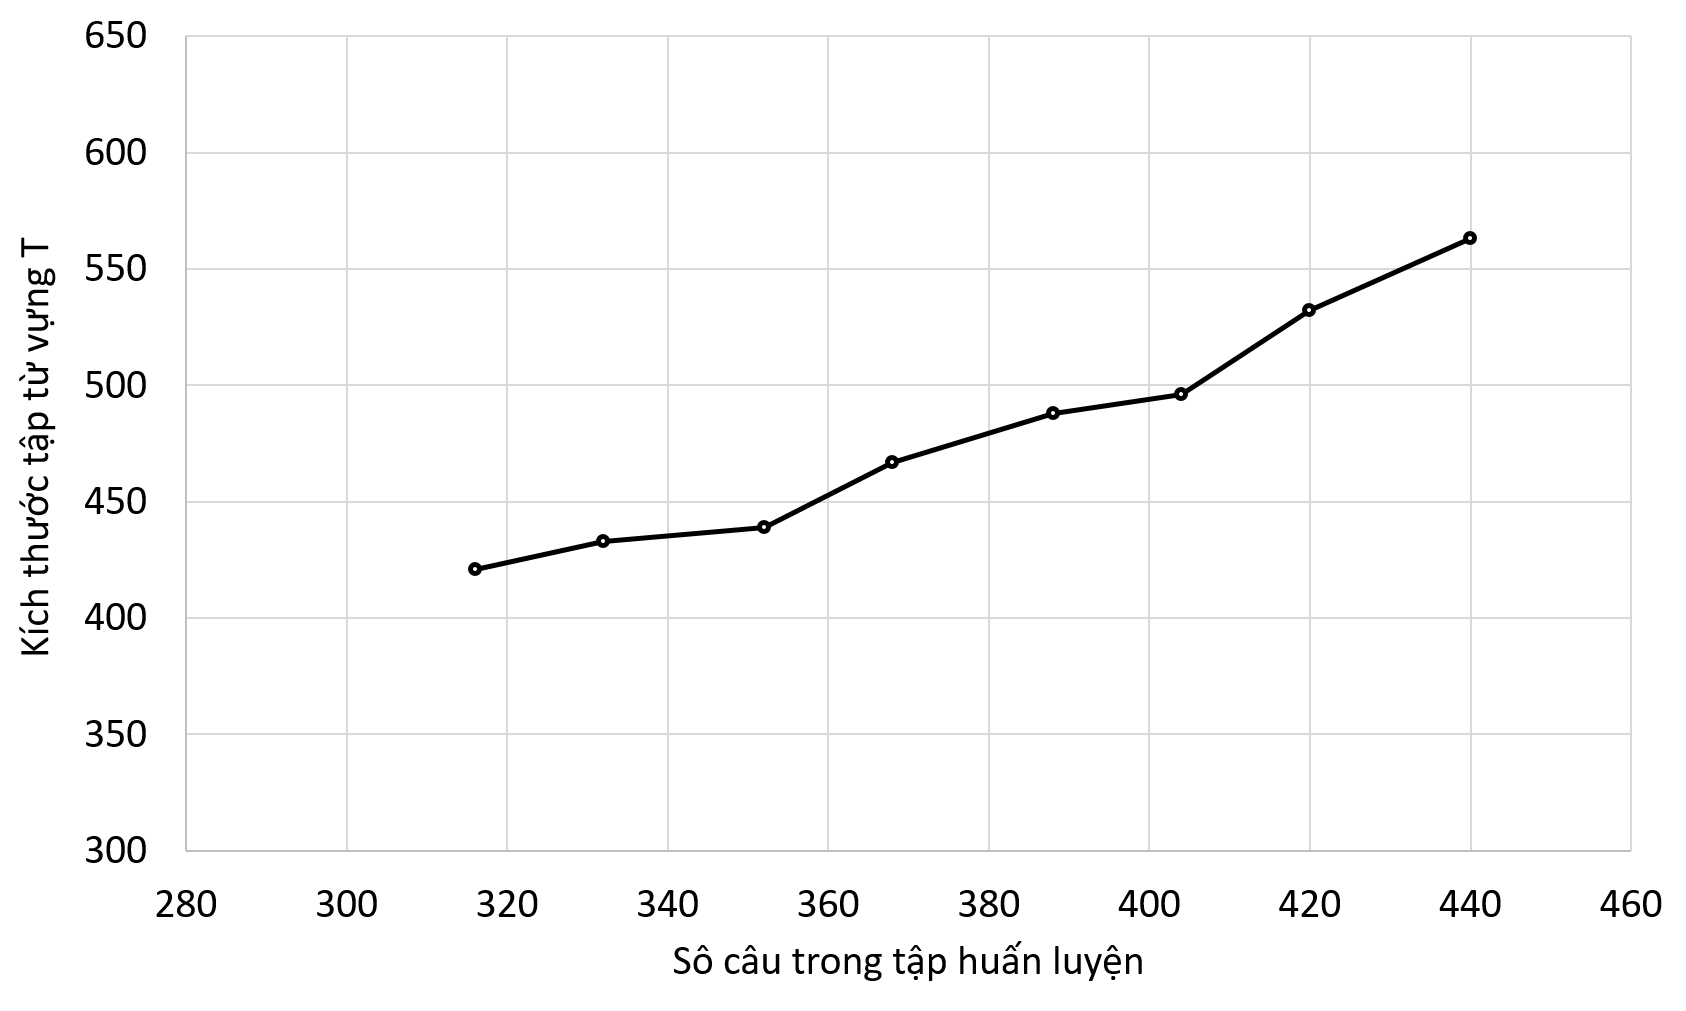
\includegraphics[scale=0.15]{../hinh/socau_vs_tuvung.png}
\caption{Mối quan hệ giữa kích thước tập dữ liệu huấn luyện và kích thước tập từ vựng T} \label{fig:so-cau-vs-tu-vung}
\end{subfigure}
~
\begin{subfigure}[h]{0.45\textwidth}
\centering
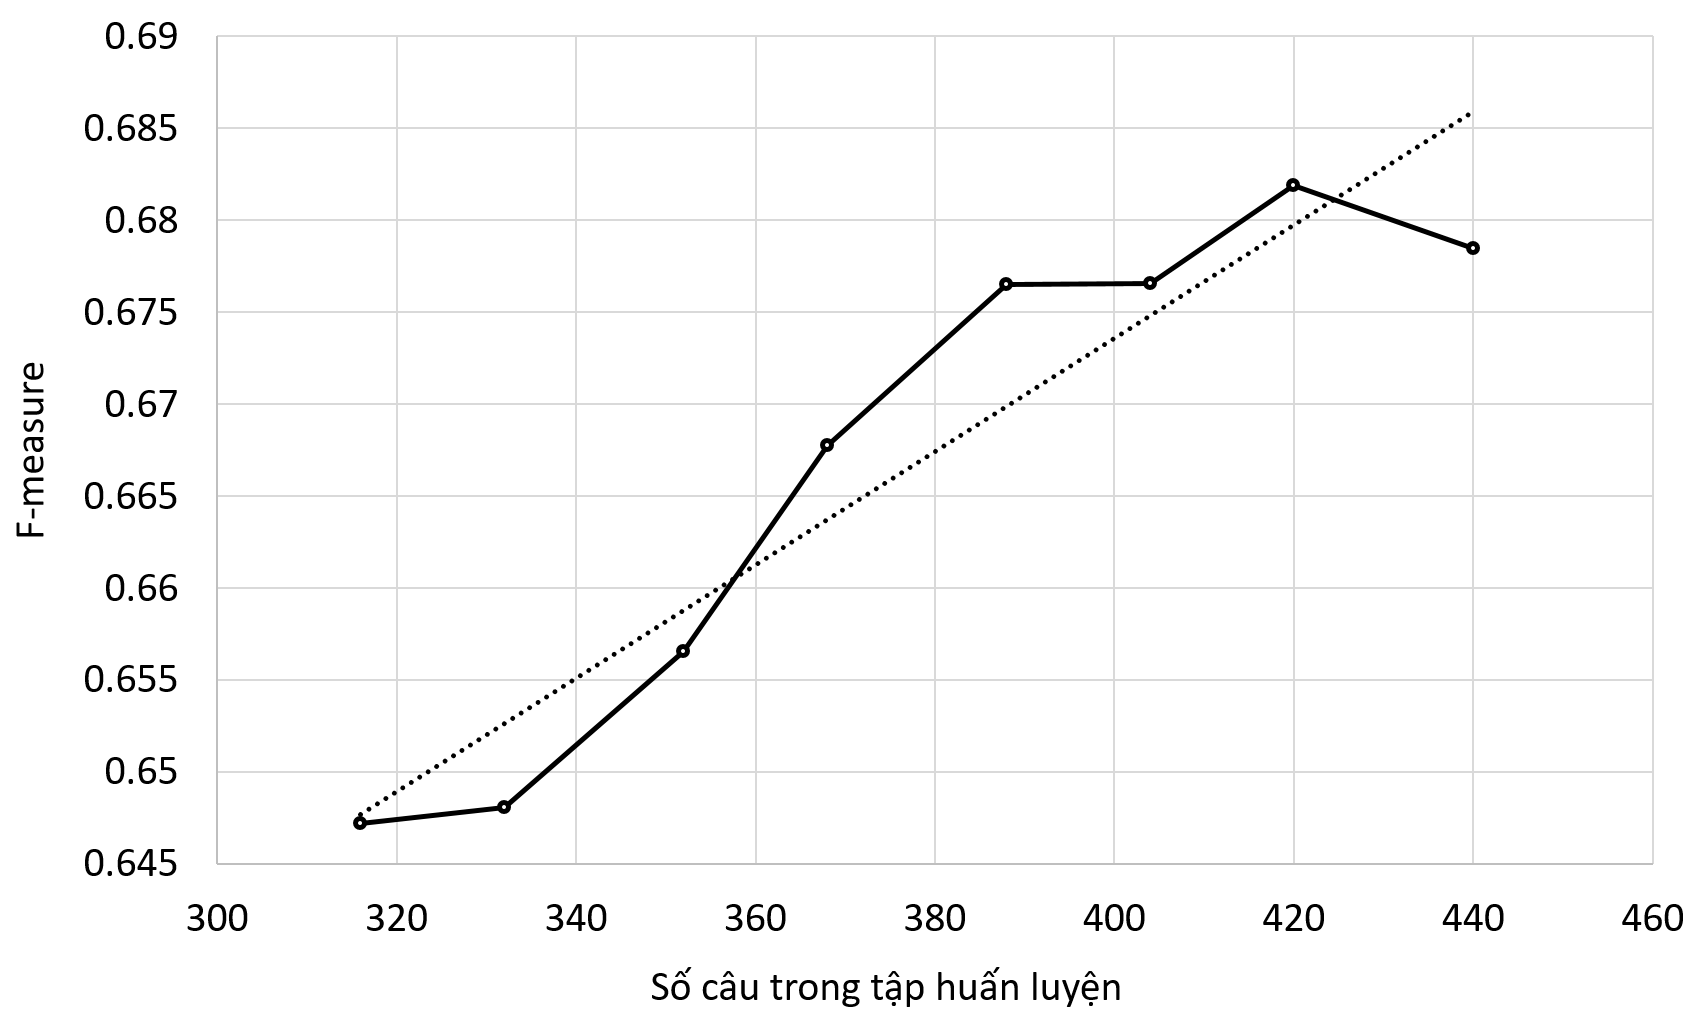
\includegraphics[scale=0.15]{../hinh/socau_vs_f.png}
\caption{Mối quan hệ giữa kích thước tập dữ liệu huấn luyện và độ đo F} \label{fig:so-cau-vs-f}
\end{subfigure}
\caption{Ảnh hưởng của kích thước tập dữ liệu huấn luyện đến đặc trưng n-gram} \label{fig:so-cau-vs-ngram}
\end{figure}

\subsubsection*{So sánh kết quả đối với từng lớp}
Chúng tôi tiến hành phân tích kết quả cụ thể đối với từng lớp. Kết quả Hình \ref{fig:p-r-f-class} sử dụng lần thử nghiệm đạt kết quả tối ưu nhất, sử dụng các đặc trưng: n-gram, change phrase, phủ định và SO-CAL. Kết quả 2 lớp \tichcuc và \trungtinh khá đồng nhất, trong khi lớp \tieucuc lại cho kết quả thấp hơn rõ rệt. Vì vậy, cần thêm các phân tích các câu thuộc lớp \tieucuc để tăng độ chính xác cho hệ thống.
\begin{figure}
\centering
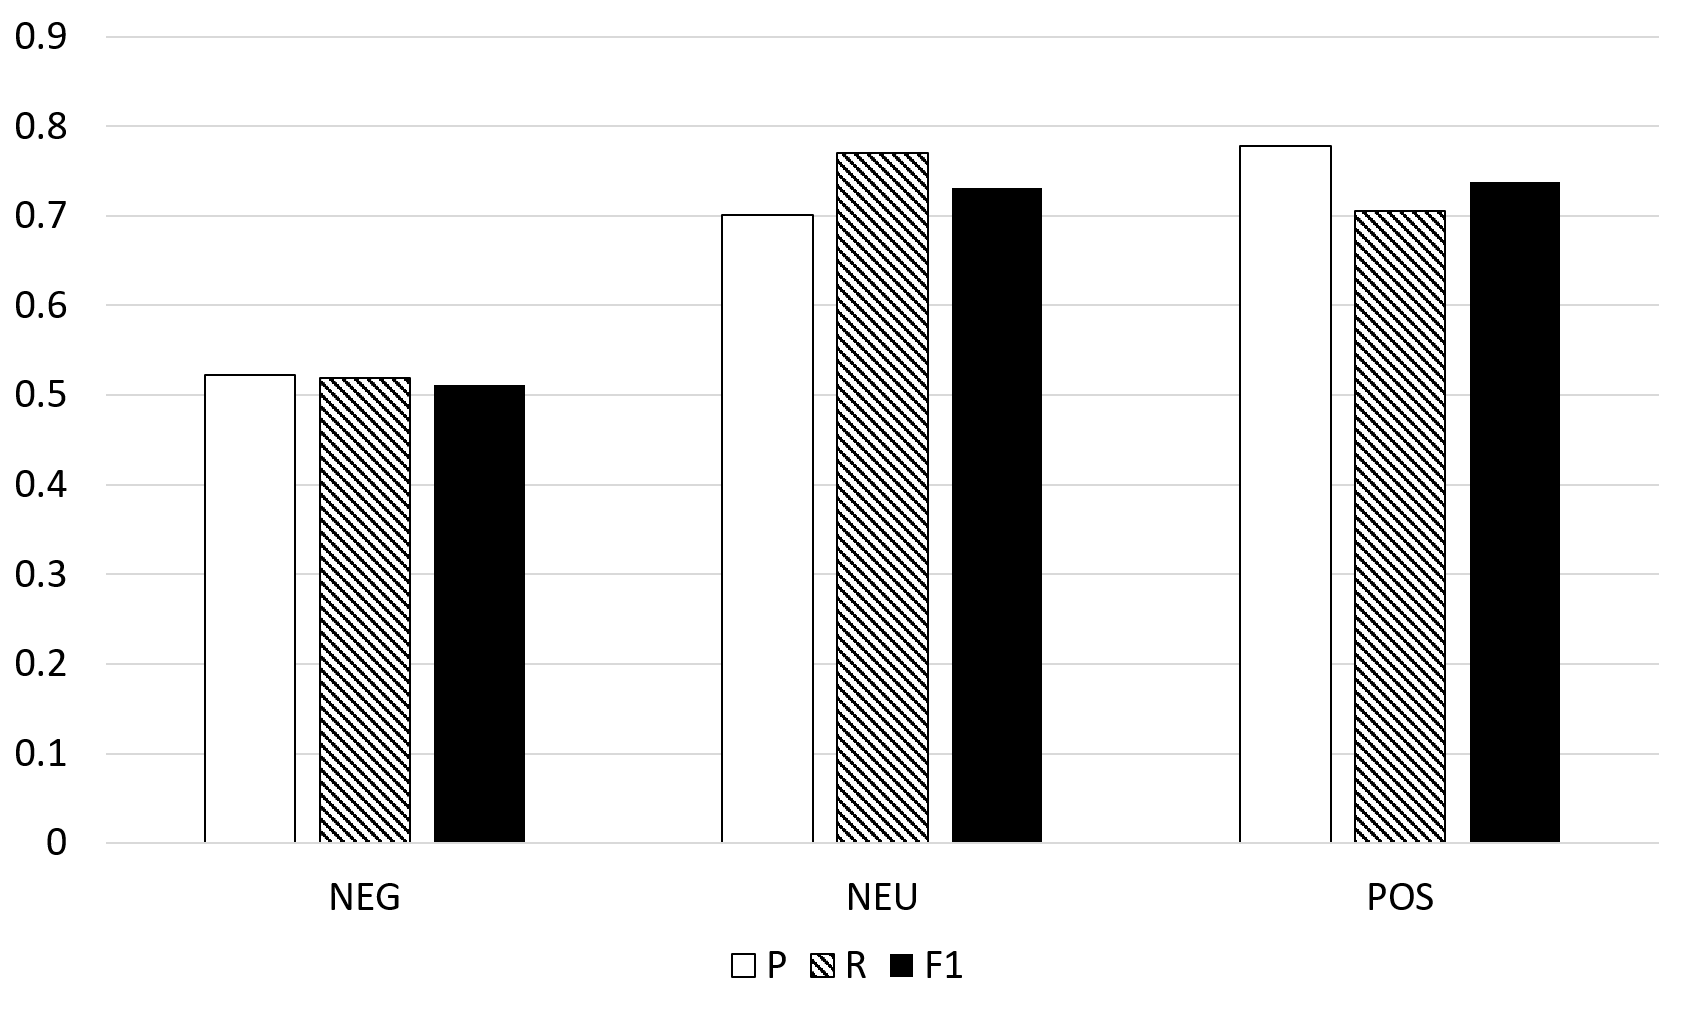
\includegraphics[scale=0.25]{./hinh/class.png}
\caption{Độ chính xác, độ bao phủ và F-measure trong từng lớp} \label{fig:p-r-f-class}
\end{figure}